\documentclass{article}

\usepackage{amssymb}
\usepackage{amsmath}

\title{ME699 Final Project Proposal}
\date{02-04-2020}
\author{Benton Clark, Ethan Howell, Brian Moberly}

\begin{document}
\pagenumbering{gobble}
\maketitle

\section{Project Outline}
For our project, we are proposing three primary phases:

\begin{itemize}
  \item Modeling
  \item Perception and Planning
  \item Control
\end{itemize}

\noindent Each phase of the project will feed into the next.
For instance, the model designed in the robotic modeling section will then be
used in the control section of the project.
By the end of the project, our goal is to have a fully modeled, controlled
robotic manipulator capable of following a simple trajectory and moving to
desired target locations in task space to accomplish simple goals.

\section{Demonstration}
The end goal of our project is to apply the modeling, perception and adaptive
controls to the Panda Robot arm.
The task will consist of the arm beginning in a configuration, moving towards an
intermediate state where an object is located, picking up that object, and
successfully moving that object to a desired goal state.
The object will be of unknown and variable mass, meaning the arm must be able to
effectively adapt to objects of differing weight online.
The exact location of the object must also be identified by the ``camera''
attached to the Panda, meaning a valid path must be found to both reach the
object and take it to the goal state.
The goal state will be fixed.

For the modeling portion, both static free and dry friction models will be used.
The perception and planning portion will be tasked with filtering out small
amounts of Gaussian white noise from both the joint configurations and the
camera readings in task space.
It must also find a valid trajectory of configurations in both task and joint
space to complete the objective.
The adaptive controller will use both the modeling and perception values in
determining the joint torques to command to follow the given trajectory.
It will also compensate for the additional weight on the last link of the arm
when the object of unknown mass is picked up.

\section{Robotic Modeling}
\subsection{Approach}

The general equation of motion for a robotic manipulator can be expressed as:

\begin{equation}
  \label{eom-manipulator}
  M(q)\ddot{q} + C(q,\dot{q})\dot{q} + G(g) = \tau
\end{equation}

\noindent where $M(q)\in\mathbb{R}^{n\times n}$ is the mass matrix of the joints,
$C(q,\dot{q})\in\mathbb{R}^{n\times n}$ is the Coriolis matrix,
$G(q)\in\mathbb{R}^{n}$ is the conservative force vector acted on the arm by
gravity, and $\tau\in\mathbb{R}^{n}$ are the torques commanded to each joint.
Each of the terms on the left hand side of the equation can be directly modeled
when the manipulator joint information is known.
However, when this information is not available, a neural network can be used to
estimate the value of these matrices.

To model the conservative force vector, a robotic manipulator can be controlled
with a simple PD controller and brought to a stop at a given configuration value
$q$.
When the manipulator is at rest, Eq. (\ref{eom-manipulator}) simplifies to:

\begin{align}
  \label{eom-manipulator-stopped}
  M(q)*0 + C(q,0)*0 + G(q) &= \tau\\
  G(q) &= \tau
\end{align}

\noindent which allows the loss function for the function approximator
$\hat{G}(q)$ to be expressed as:

\begin{equation}
  \label{loss-function-gq}
  \hat{G}(q) - \tau = \delta_{Loss}
\end{equation}

To model the mass matrix with a function approximator $\hat{M}(q)$, we must
again model a loss function to train the network.
This proves more difficult, as the mass matrix must be isolated on the left hand
side of the equation.
However, if the number of acceleration samples taken at a given configuration
$q$ satisfy $rk(M(q)) = n_{samples}$, we could then construct an acceleration
matrix $\ddot{Q} = [\ddot{q_{1}}, \ddot{q_{2}}\dots\ddot{q_{n}}]$ which
satisfies $rk(\ddot{Q}) = rk(M(q)) = n$.
Properties of linear algebra now guarantee that a unique inverse of this matrix
must exist, and the equation can then be expressed as:

\begin{align}
  \label{eom-manipulator-accel}
  M(q)\ddot{Q} + C(q,\dot{Q})\dot{Q} + G(q) &= \tau\\
  \label{eom-manipulator-accel-m}
  M(q) &= \ddot{Q}^{-1}(\tau - G(q) - C(q,\dot{Q})\dot{Q})
\end{align}

The problem with this method is that the Coriolis term is still in place, and we
have no estimate for this value.
However, if we take our $\ddot{q}$ samples at the initial point when we first
begin accelerating, we should see that $\dot{q} \approx 0$, and thus Eq.
(\ref{eom-manipulator-accel-m}) can be expressed as:

\begin{align}
  M(q) = \ddot{Q}^{-1}(\tau - G(q))
\end{align}

\noindent which now allows for a loss function to be formulated.

For the Coriolis matrix, it directly depends on the mass matrix $M(q)$, and thus
once an estimate for $M(q)$ is formulated, the Coriolis matrix can be derived
from the given values of the $\hat{M}(q)$ matrix.

\subsection{Experiments}
The experiments for this section will include learning both $\hat{G}(q)$ and
$\hat{M}(q)$ using the proposed method above in two settings: One in a friction
free environment, and another when static friction is present.
The friction free case will be used primarily as a base case, and the accuracy
of both the $\hat{G}(q)$ and $\hat{M}(q)$ will be compared to their true values.
This will serve to see how effective this method is in general, as
friction begins complicating the process.

The frictional case will be further broken down into two sections.
The first will consist of learning the two maps without static friction
compensation, and the second will include static friction compensation.
Static friction will be modeled as a constant $\mu_{s}$, so this can easily be
added into the above formulations (primarily for the mass matrix case).

\section{Perception and Planning}
\subsection{Uncertainty in Configurations}
The robot configuration $q_1$, $q_2$, ..., $q_n$ determines how the robot will
interact with the task space and the end-effector.
Assuming that the end-effector has a camera on its end and can understand its
surroundings, the perception through said camera will be used to achieve motion
and interaction with an object in the task space.
A combination of the RRT path planning algorithm, Kalman filtering, and
Forward/Inverse kinematics will lead to the configuration that the robot is in
to have the end-effector reach the object.
An object with some mass $M_o$ will be placed in the task space.
The robot's purpose is to move to the object, pick it up, and move it to a
desired position.

\subsection{Approach}
The end-effector perception problem requires many disciplines of robotics.
First, a landmark based Kalman filter will be applied to the robot.
This will test our ability to move to the object.
Then, applying kinematic theory, the configuration of the robot to achieve the
end-effector location and orientation corresponding to the object will be
achieved.

\subsection*{Control Models}
To validate our control models, it is important to evaluate the error dynamics associated with the controllers. To do this, we begin with the comparison of the error convergence between the Adaptive Control model and the classical PD Control model. This comparison was made with a fixed, known weight, as well as no noise in the joint values.
\begin{figure}[H]
	\centering
	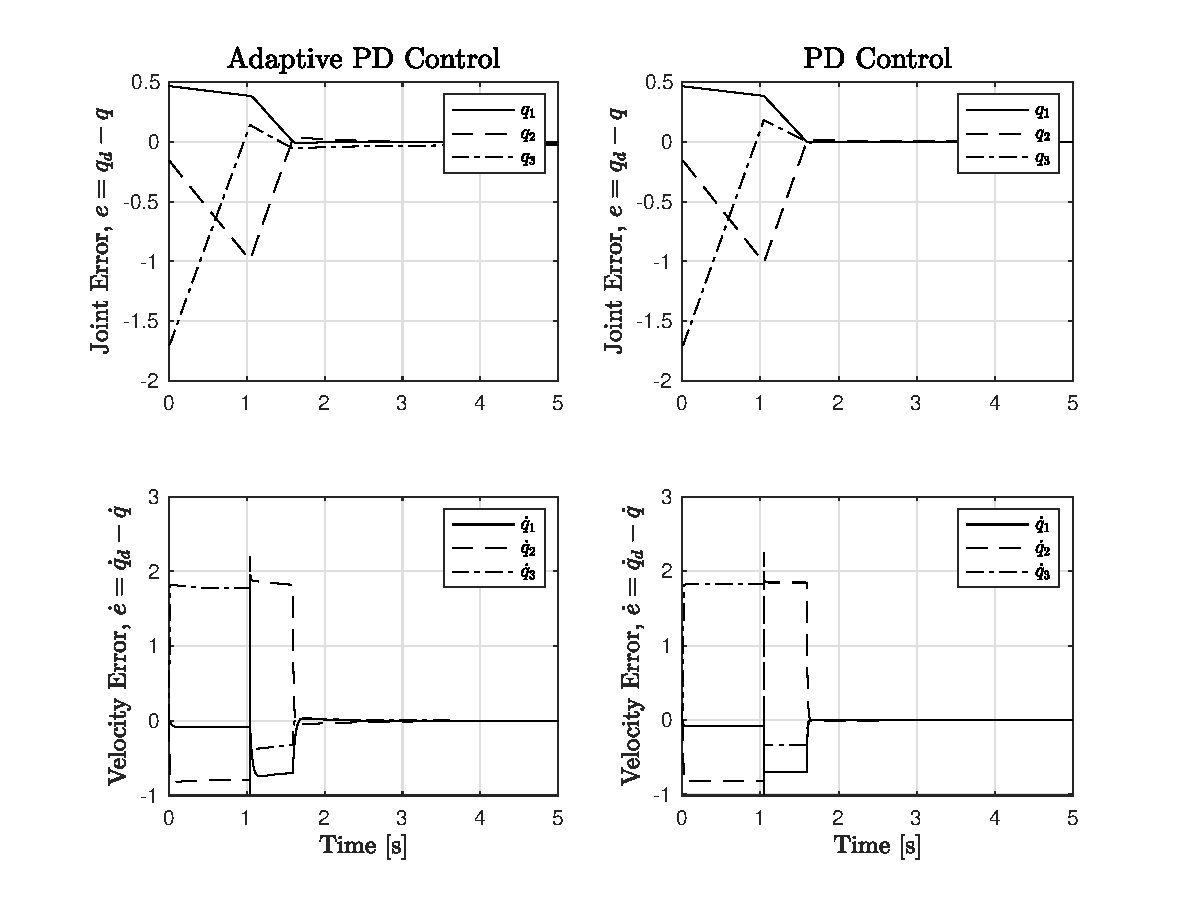
\includegraphics[width=0.7\textwidth]{figures/adpdErr.eps}
	\caption{Convergence of controller error dynamics}
	\label{fig:adpderr}
\end{figure}
As shown in Fig. \ref{fig:adpderr}, both controllers converge to the steady state value of zero in approximately the same time. One benefit to adaptive control however, is that as the mass changes (i.e. an object is picked up), the adaptation law accounts for the change in mass. With PD Control, there is no way to account for this mass addition and an increase in error is introduced.\\

We then evaluate each controller by it's ability to follow the desired trajectory provided by the $RRT^{*}$ path planning algorithm.
\begin{figure}[H]
	\centering
	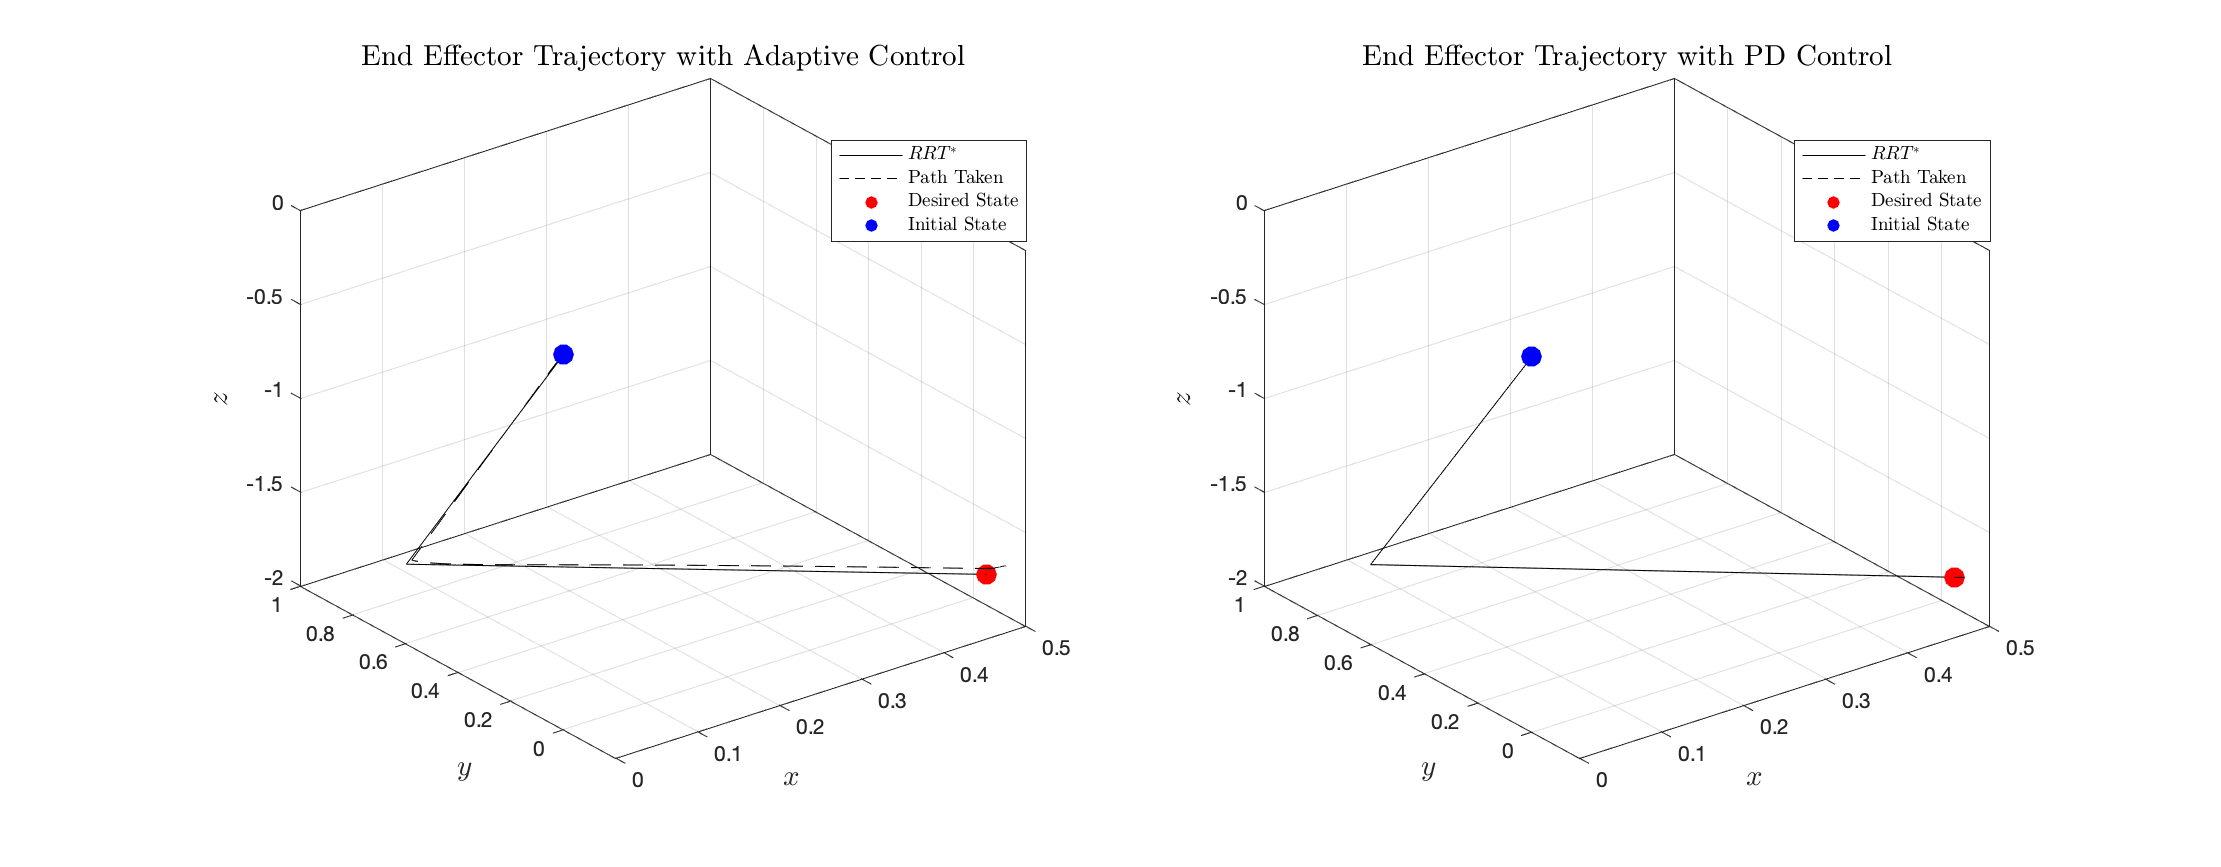
\includegraphics[width=0.9\textwidth]{figures/eeTraj.eps}
	\caption{Desired end-effector trajectory vs actual}
	\label{fig:eetraj}
\end{figure}
We can see from Fig. \ref{fig:eetraj} that in this case, the PD Controller maintains the desired trajectory more tightly than the Adaptive Control model. However, the error between the two control models is of an insignificant degree, thus the adaptive control model is chosen for the simulation.


\section{Team Contributions}
For the individual sections of the project, Benton will focus on the robotic
modeling, Ethan on the robotic controls, and Brian on the perception and
tracking.
However, since each part of the project will slowly feed into one another, each
team member will help contribute to all three parts of the project equally.

\end{document}
